\scanpage{12}
\[
n\left\{\begin{array}{ll}L&d\text{ gén.}\\\cup&\\L'&d'\text{ gén}\end{array}\right.
\qquad\begin{gathered}(d'-1)=n(d-1)\\2=2.1\end{gathered}
\qquad\textcircled{1}
\]

\figure{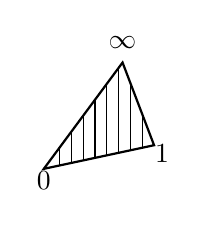
\begin{tikzpicture}
\draw[thick] (0,0)--(1,1.35)--(1.4,.3)--cycle;
\foreach \x in {.2,.35,.5,.65,.8,.95,1.1,1.25}{\draw (\x,{.214*\x})--(\x,{min(1.35*\x,3.975-2.625*\x)});}
\node at (0,-.15) {$0$};\node at (1.5,.2) {$1$};\node at (1,1.6) {$\infty$};
\end{tikzpicture}}

\figure{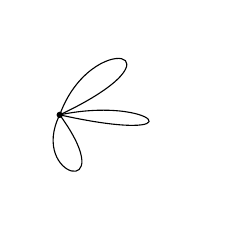
\begin{tikzpicture}
\draw (0,0)..controls(.4,1.1)and(1.7,.8)..(0,0);
\draw (0,0)..controls(1.2,.25)and(1.8,-.4)..(0,0);
\draw (0,0)..controls(-.4,-.8)and(.8,-1.1)..(0,0);
\fill (0,0) circle(.04);
\end{tikzpicture}}

\[
\begin{array}{lll}L\simeq\pi_1(X)&&1-d\\\cup&&\\L'\simeq\pi_1(X')&&1-d'\end{array}
\]
\[
\pi^+
\]
\diagram{\begin{tikzcd}[ampersand replacement=\&,column sep=small,row sep=small]
\rho_0\arrow[d]\&\rho_1\arrow[dd]\&\rho_\infty\arrow[d]\\
\rho_0^{-1}.\&\&\rho_\infty^{-1}\\
\&\rho_\infty\rho_0\&
\end{tikzcd}}

\[
\pi
\]
\diagram{\begin{tikzcd}[ampersand replacement=\&,column sep=large,row sep=large]
\&\&\margin{\text{avec }\varinjlim}\\
\operatorname{Ens}(\pi)\arrow[r,"\begin{gathered}F\\\text{commutant}\end{gathered}","\text{aux }\varinjlim"']\arrow[d,leftrightarrow]\&C\arrow[r,bend right=12,"G\text{ commute}","\text{aux }\varinjlim"']\arrow[ur,bend left=15]\&C'\\
\phantom{X}\&X\quad\pi\text{-objet }\inserted{\text{à droite}}\text{ de }C\&
\end{tikzcd}}
\margin{$(\simeq\operatorname{Ens}/\pi))$}

\[
F\longmapsto F(\underline{\pi_s})
\]
\[
X\longmapsto F_X:E\longmapsto\underbrace{X\times_\pi E}_{\in\operatorname{Ob}C}
\]
\[
\operatorname{Hom}_C\bigl(X\times_\pi E,
\underset{\substack{\rotatebox{90}{\ensuremath{\in}}\\\operatorname{Ob}C}}{\deleted{E}\inserted{\unsure{Y}}}\bigr)
\simeq\operatorname{Hom}_\pi\bigl(E,\operatorname{Hom}(X,Y)\bigr)
\]
\[
E\simeq\coprod_{i\in I}\pi/H_i
\]
\[
X\times_\pi E=\coprod_i\underbrace{X\times_\pi(\pi_s/H_i)}_{X/H_i}
\]

\mspage{11}
